\section{Architectural Design}

%  in automatico Section [number]
\subsection{Overview}
\begin{figure}[H]
          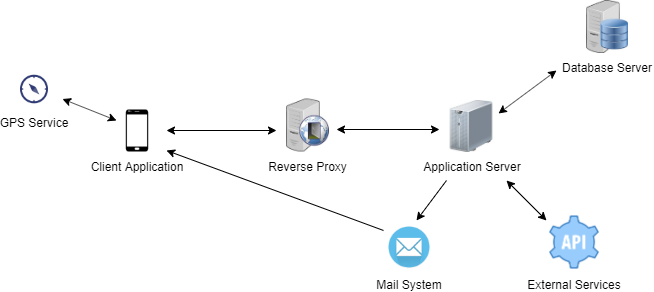
\includegraphics[scale=0.54,left]{Images/overview.png}
        \caption{System overview}
\end{figure}
The above figure shows an high level overview of the System's architecture.\\
We can immediately identify that is divided in two parts: the Client Application part and the Application Server part.\\
The former shows the service used by the Client Application and its communication with the Application Server.\\
The other one indicates how the System works with the external functionalities in order to accomplish the required Goals.\\
Further details on the System components and their interactions will be explained in detail in the following sections.

\subsection{Component view}


\begin{figure}[H]
\centering
\advance\leftskip-6cm
          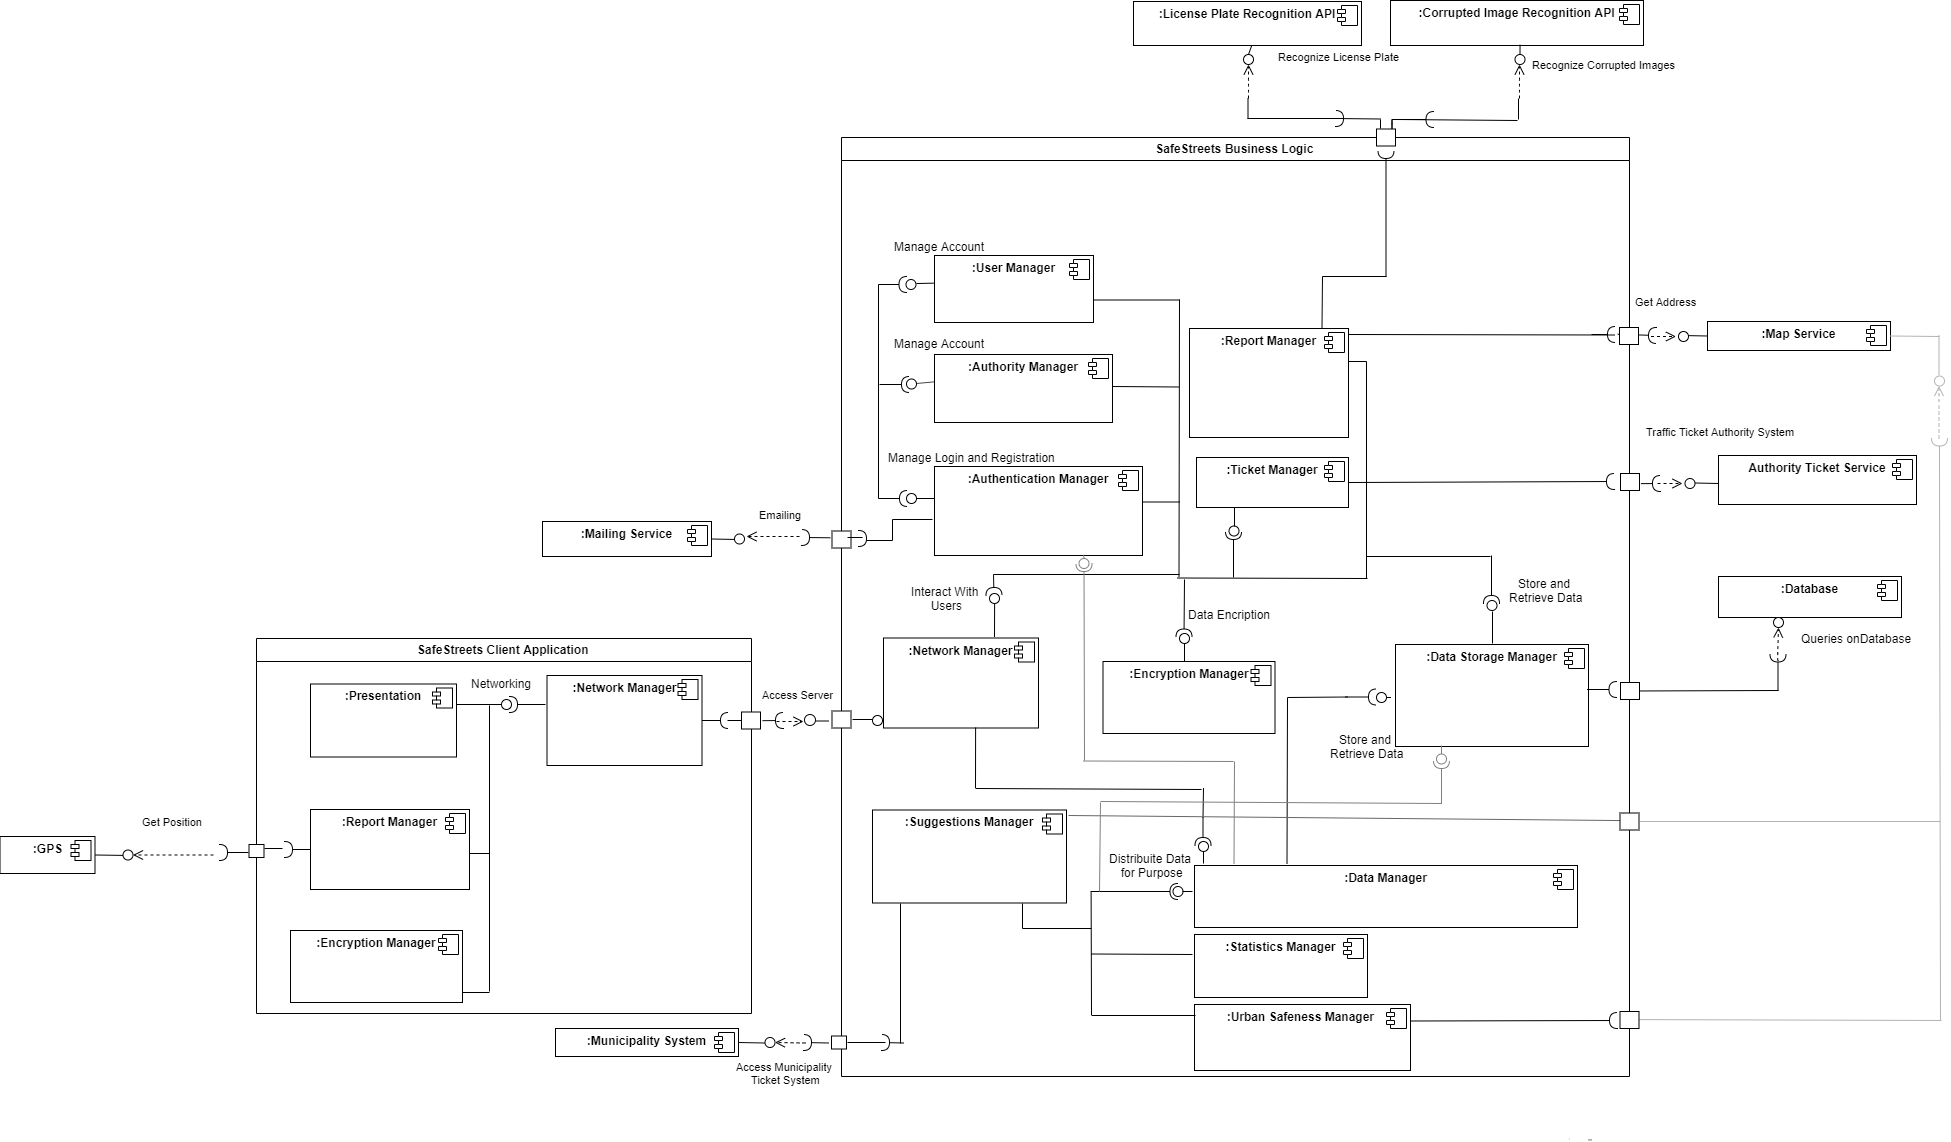
\includegraphics[width=1.5\textwidth,left]{Images/Component_view.png}
        \caption{Component Diagram}
\end{figure}


In this section, an UML diagram is used to show the internal structure of the \textit{SafeStreets} system. \\
It is divided into one application client layer and one Business Logic layers, which reflect the physical structure showed in the Overview.
The client layer communicates with the Business layer for requesting the services and accomplishing its scopes. 
Business Logic Layer communicates with the Database, from which it stores and retrieves data.\\
The relationships and interfaces between the components are represented in our diagram through assembly connectors and delegation connectors (externally).
Let's now take into account each single component:\newline

\noindent\textbf{SafeStreets Business Logic}\\
This component is delegated to solve all the tasks relative to the processing of new reports, the managing of reports in general, and to provide all the functionalities about Traffic Ticket generation, Statistics, Suggestions and Urban Safeness.\\
Furthermore, also the responsibilities of registration and authentication tasks lie here. 
\begin{itemize}
    \item \textbf{Authentication Manager}\\
    This component is in charge of managing the registration tasks, so it will check the data of the users, add them to the Database, send confirmation emails. It is also up to this component the task of logging users in, giving them the right authorizations.  
    
    \item \textbf{Network Manager}\\
    Every communication among the Server and the Clients go through this component; it routes incoming messages toward the right component, and sends outgoing messages at the recipient application client.
    
    \item\textbf{User Manager}\\
    It handles the functionalities of User accounts. Through the presentation level it provides the right interface to the User. Furthermore, this component handles the access and modification to the User's personal data, username and password. 
    
    
    \item\textbf{Authority Manager}\\
     It handles the functionalities of Authority accounts. Through the presentation level it provides the right interface to the Authority. Furthermore, this component handles the access and modification to the Authority's personal data and password. 
     
     \item \textbf{Report Manager}\\
     This component takes care of all the aspects of the reports management.
     It takes incoming reports from Users, and check if they correspond to already notified violations. It uses external service API to check if the received picture has been corrupted, and API to recognize the license plate from the picture. An external Map Service is used to obtain the address from the position of the report. This component handles the modification or deletion operations of the Users.\\
     Report Manager is also in charge of computing the trustness of each report, and deciding if to discard it or no, and in case, it must store it correctly in the Database.\\
     Operations of viewing, accepting or rejecting a report, carried out by Authorities, are also under the responsibility of the Report Manager.
     Report Manager also ensures that no more that one Authority at a time can access a report.
     
     
     \item\textbf{Ticket Manager}\\
     After that a report has been accepted by an authority, the Application Server generates a traffic ticket related to that violation. All that concerns the managing of traffic tickets is handled by the Ticket Manager. It allows to generate tickets, by accessing the external Authority Ticket Service.
     
     \item\textbf{Data Store Manager}\\
     This component realizes a intermediate layer between the Database and each component that accesses it; it provides to these components an easier way to store and retrieve data from the Database. \\
     Data Store Manager create queries and directly interacts with the Database. \\
     It is linked to every other component who needs to access the Database.
     
     \item\textbf{Encryption Manager}\\
     Components who manage important data interfaces with the Encryption Manager, who provides encryption methods.
     
     \item\textbf{Data Manager}\\
     The Data Manager stands between the Suggestions, Statistics and Urban Safeness managers, and the rest of the Logic Layer; these three components only use stored data to provide information based on the kind of request from the client. Data Manager gets the request, and chooses to which of these components turn the request to, depending on the type of information requested. \\
     But the main scope of this manager is to keep updated the three components under it; it implements an Observer Pattern which receives a pull notification every time reports or tickets are added to the Database, then it brought up to date the components information that are interested in the new data. 
     
     \item\textbf{Suggestion Manager}\\
     This component accesses the external Municipality data and crosses them with the data of SafeStreets. In order to provide physical intervention at the urban mobility this component also exploits the external Map Service.
     It stores the suggestions in the Database. Through the Data Manager, the Suggestion Manager keeps its suggestions updated to every new incoming data.\\
     Furthermore, through the Presentation layer it allows Authorities to view the suggestions list.
     
     \item\textbf{Statistics Manager}\\
     Handles the statistics information that Users and Authorities view in the Statistic Section of the client application.\\
     It accesses the Database, retrieves information, computes statistics, and keep them up to date thanks to the Data Manager.
     
     \item\textbf{Urban Safeness Manager}\\
     It elaborates data from the Database to identifies the most safe or unsafe areas, and then present them to Users and Authorities by using the external Map Service.\\
     As other components, it leans to the Data Manager to keep its information updated to every new data.
     
\end{itemize}

\noindent\textbf{External Interfaces}\\
Both Client Application and Business Logic Layer use functions form external component with which they communicate. We are introducing these components with some more particulars:

\begin{itemize}
    \item \textbf{GPS}\\
    Global Positioning System, is used by the Client Application to send, along with a report notification, the global position where the violation occurred.\\
    Obviously the device on which SafeStreets is running has to have a built-in GPS module. GPS position is mandatory in a report notification.
    
    \item\textbf{Map Service}\\
    It's used by SafeStreets to retrieve the address from the GPS position, or to graphically show on a map some information requested by Users or Authorities.
    
    \item\textbf{Mailing Service}\\
    Authentication Manager uses this service to send confirmation e-mail to new registered Users, and to carry on any other via mail needed communication.
    
    \item\textbf{Database}\\
    Where SafeStreets store all its data. It is external to the Business Logic Layer, and the Data Store Manager is in charge of making this layer communicate with the DBMS running on the Database. 
    
    \item\textbf{Authority Ticket Service}\\
    Is the hardware and software system owned by Authorities through which Authorities generates traffic tickets. SafeStreets accesses this system and its functionalities to correctly generate tickets.
    
    \item\textbf{Municipality System}\\
    For providing suggestions, SafeStreets need to cross its own data with urban data owned and provided by the municipality. \\
    This data are obtained by making Suggestions Manager access the Municipality System that contains the data.
    
    \item\textbf{License Plate Recognition API}\\
    Report Manager has to add metadata to the received report notification.
    In order to get the License Plate of the vehicle involved  in a violation, SafeStreets must use an algorithm that recognize it from the picture received.\\
    This algorithm is provided from an external API.
    
    \item\textbf{Corrupted Image Recognition API}\\
    Corrupted data that is received must be discarded. SafeStreets (and in particular, the Report Manager) uses ad external API service that implements an algorithm to identify modifications carried out on a picture.
    
\end{itemize}


\subsection{Deployment view}
The distribution of components capturing the topology of the system is illustrated below by using a deployment diagram.\newline
The system is structured in a multitier architecture.
\newline
\begin{figure}[H]
\centering
          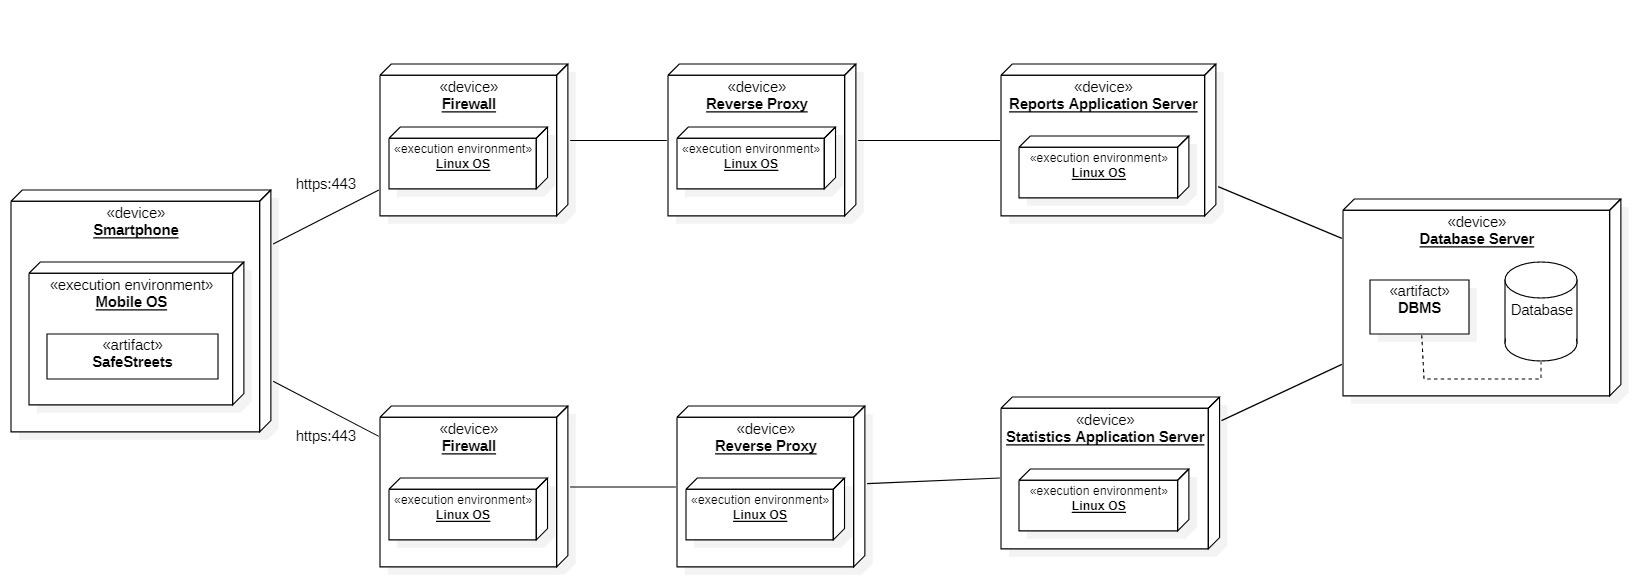
\includegraphics[width=1.25\textwidth,left]{Images/deployment_diagram.png}
        \caption{Deployment Diagram}
\end{figure}

\noindent\textbf{Mobile Device}\newline
This node represents the mobile device of the User or Authority, both can access to the functionalities of SafeStreets by using their own device.\\

\noindent\textbf{Firewall}\newline
This component allows to protect the Reverse Proxy by filtering the packets received from \textit{Internet}.\newline

\noindent\textbf{Reverse Proxy}\newline
We chose to deploy a reverse proxy in order to increase parallelism and scalability. Moreover, the reverse proxy is in charge of the load balancing since it is the component receiving all the request from internet (filtered by the Firewall). Another reason for the deployment of the Reverse Proxies is because it increases security and anonymity by protecting the identity of our backend servers.\\

\noindent\textbf{Application Server}\newline
This component contains all the logic used to accept reports from Users, allows the corresponding Authorities to view them, computes statistics by accessing to local and public information about traffic violations, generates suggestions and allows to visualize safe/unsafe areas. In order to balance the workload this component may be replicated.\newline

\noindent\textbf{Database Server}\newline
This part of the System is equipped with a relational DBMS, it allows to store and retrieve all the data needed by the Application Servers.

\subsection{Runtime view}
\subsubsection{Proxy Runtime View}
The sequence diagram in \textit{Figure 3} illustrates the interaction between the User, the Reverse Proxy and a component of the Application Server. Everytime a User sends a request through the client mobile application, the Reverse Proxy verifies if the request follows the proper scheme that defines a SafeStreet's client request, if the verification fails it returns an ERROR message to the client, otherwise it selects the correct server component to forward it. The Reverse Proxy could have been used to perform a verification of the credentials of the User but it was preferred to save a token in the Database and perform a query every time through the Data Storage Manager. In all the following diagrams the interaction between the User and the Reverse proxy won't be included for readability purposes, but it should be kept in mind that all the external requests will pass through the Reverse Proxy and only the ones with a correct schema will be forwarded as HTTP requests.
\begin{figure}[H]
          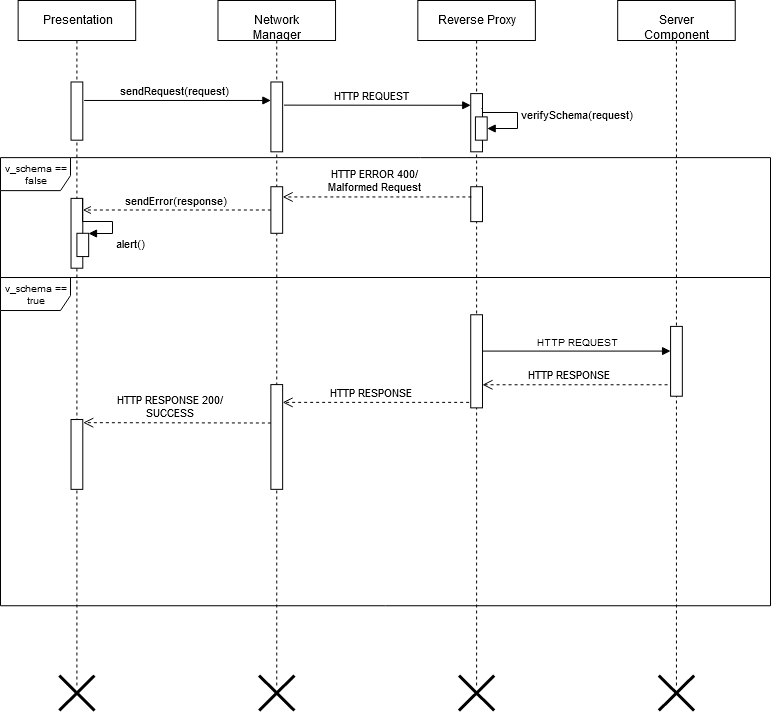
\includegraphics[scale=0.55]{Images/seq_proxy2.png}
        \caption{Proxy Runtime View}
\end{figure}

\subsubsection{Registration Runtime View}
A Guest to use \textit{Safestreets} functionalities need to be authenticated, so he/she must compile a registration form.\\
The Client Application provide to the Guest a form that he/she must fills with the necessary information.\\
The information are serialized and then sent to the Application Server through an HTTP POST request. The request passes through the Network Manager of the Client and of the Server, but these steps are implicit and not shown in the sequence diagram also for readability reasons.\\
The Authentication Manager handles the request, verifies if the information are correct and complete, then, through the Data Storage, invokes a Query and creates a new entry in the User table on the Database.\\
At this point the User Account has been created but it has to be confirmed. An email with a confirmation link is sent by the external Mailing Service.\\
When the Guest clicks on the provided link, a Query on the database is executed and the new credentials become active.
\begin{figure}[H]
          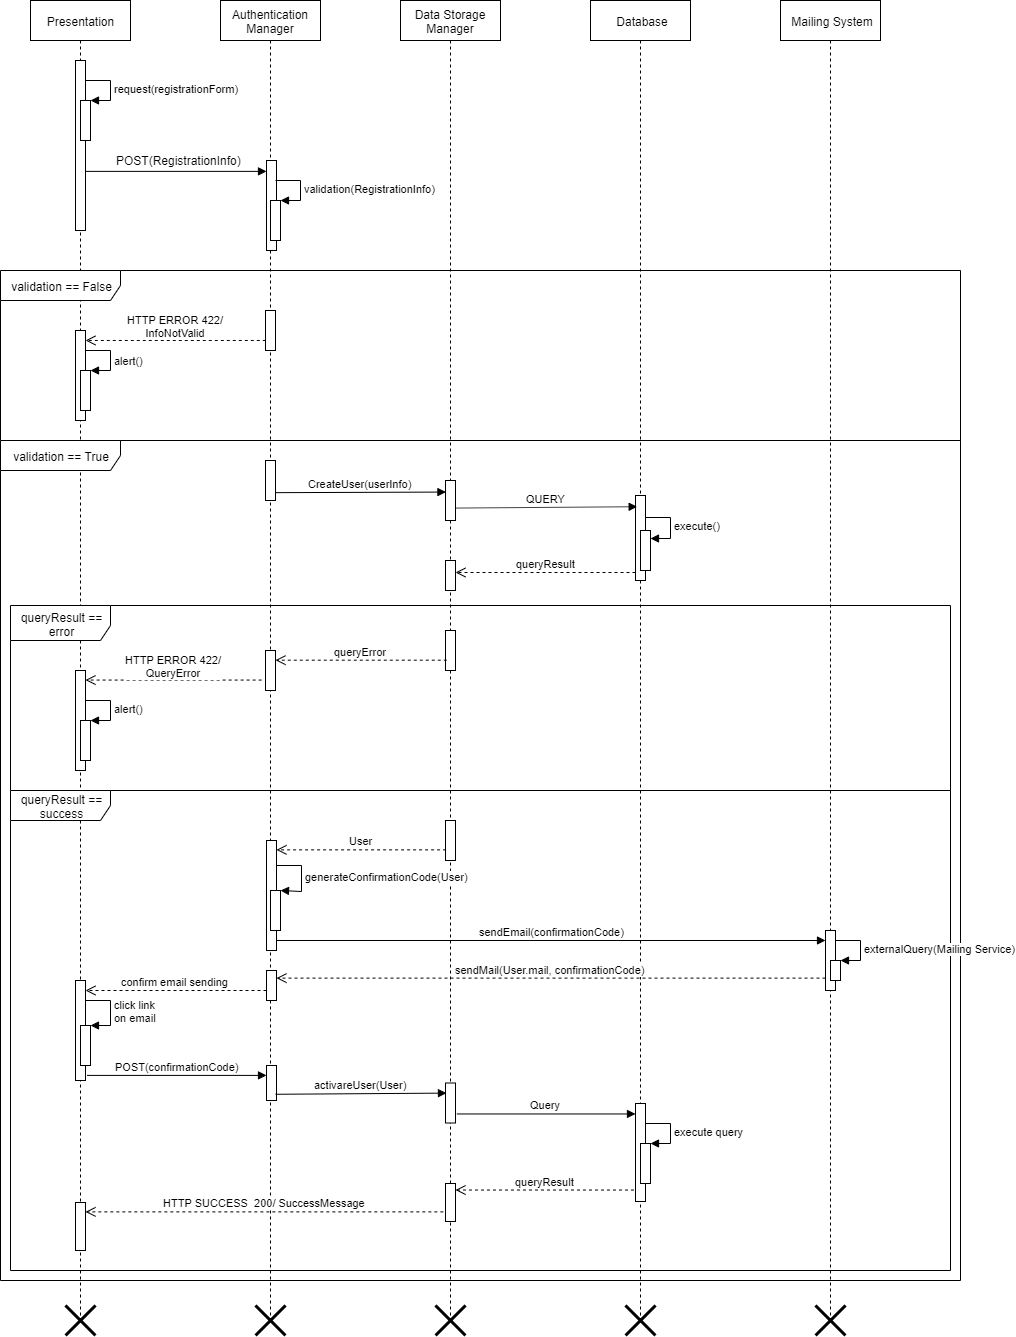
\includegraphics[scale=0.4]{Images/Seq_registration.png}
        \caption{Registration of a User Runtime View}
\end{figure}

\subsubsection{Login Runtime View}
The following sequence diagram shows the interaction between the User when he/she tries to login.\newline
As a first step, the User (through the mobile application) submits an HTTP POST request containing his/her credentials. Then like the first step in the Registration sequence diagram, the Authentication Manager receives the request and checks if the information given are correct (in terms of data types) and complete.\newline
If the validation fails, the Authentication Manager replies to the User with an ERROR response allowing the mobile application to show an alert.\newline
Otherwise, if the validation succeeds, the Authentication Manager, through the Data Storage Manager, performs a query to the Database. Then, if the number of tuples received is not equal to one, it returns a error message allowing the user to know that the username or password were incorrect, if the number of tuples is equal to one then the Authentication Manager generates a token that will allow the Server components to know that the user is logged in, this token is saved in the Database in order to validate it every time a request arrives. 

\begin{figure}[H]
          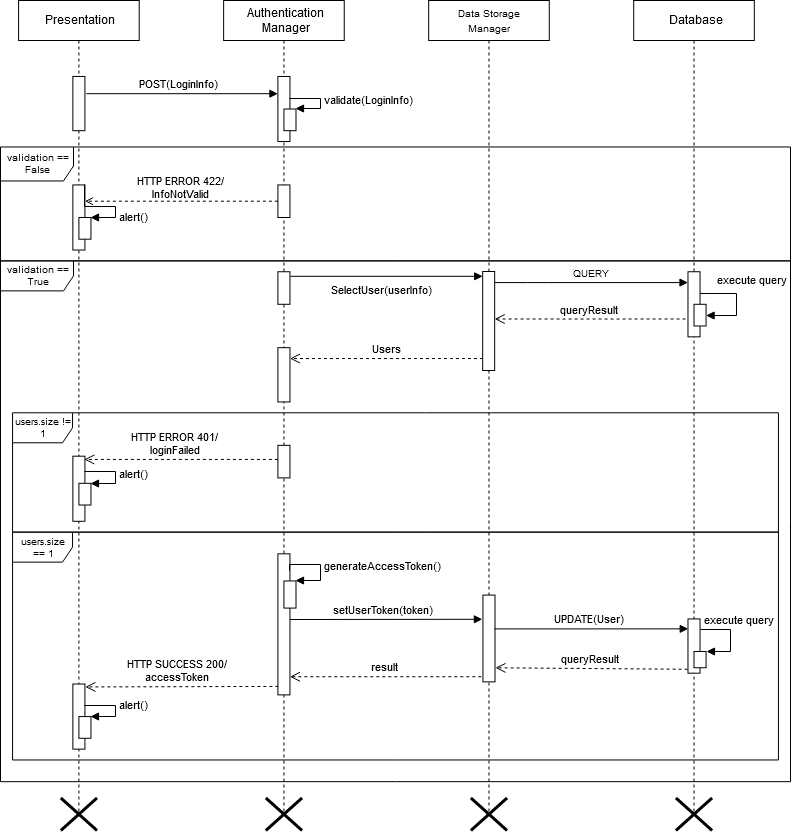
\includegraphics[scale=0.5]{Images/seq_login_definitivo.png}
        \caption{Login of a User Runtime View}
\end{figure}

\subsubsection{Send Report Runtime View}
The following sequence diagram describes the operations done by the components of the System to create and store a Report sent by a User.\\
The first step the System does is to check if the one who send a Report has the necessary privileges to send it (it need to be registered as User). After that, the Report Manager will receive all the submitted data and, after a consistency check on them is done at client level, it will add more data using external services. These services add data about the License Plate of the vehicle, the address of where the violation has occurred and the validity of the submitted photo. If some of these data has already been inserted by the User who sent the Report, the System computes its results anyway and checks if are the same, if not then the System will add some notes to the Report in which it says to Authority that some data may not be correct at all.\\\\
The appointed services are:
\begin{itemize}
    \item \textit{Map Service}, to extract the address from the position
    \item \textit{License Plate Recognizer API}, to read the License Plate of the vehicle from the provided photos
    \item \textit{Corrupted Image Recognition API}, to be sure that the received images have not been modified
\end{itemize}

\noindent Finally the complete Report is add to the Database and a confirmation of success is sent to the client.

\begin{figure}[H]
          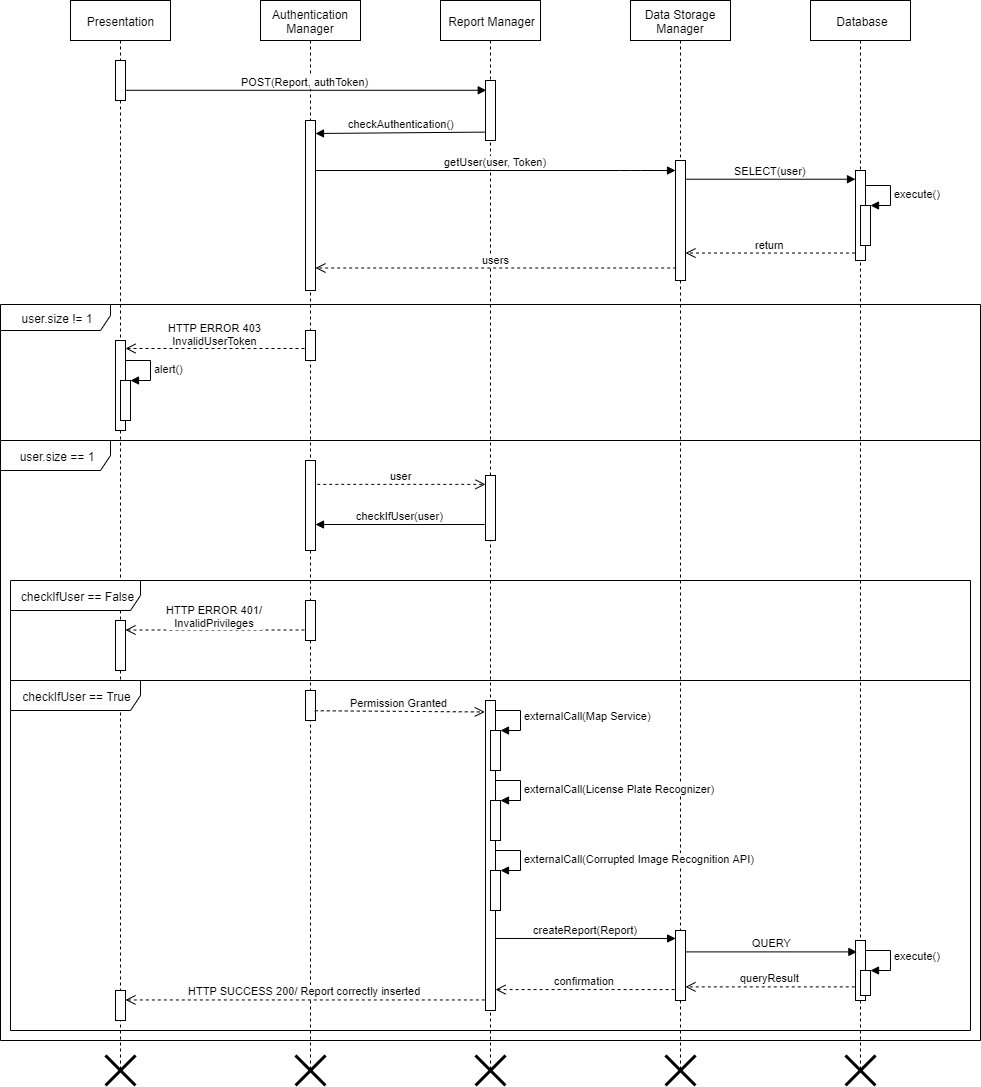
\includegraphics[scale=0.4]{Images/Seq_sendReport.png}
        \caption{User send a violation Report Runtime View}
\end{figure}

\subsubsection{Generate Traffic Ticket Runtime View}
The sequence diagram below shows the RunTime view of the generation of a Traffic Ticket, like in the previous RunTime View the first steps are used to verify if the user exists and has a valid authentication token. The difference here is that the verification steps are started by the Report Manager since the User requests the Reports Lists, Once the Report Manager gets the User instance it asks to the Authentication Manager if it is an Authority. If the verification results \textit{False} it returns a ERROR message to the User who sent the initial request. If the verification is \textit{True} then it invokes a query, through the Data Storage Manager, that allows to get the Reports corresponding to Authority's municipality.\newline
The Authority that wants confirm/reject a real violation, sends a request to get the details of that report. Once he/she has seen the details as photo, license plate, type of violation and, eventually, notes added by the Report Manager, he/she can choose to confirm or reject the report through a new POST request containing the decision and the reportID that will be send to the Ticket Manager.\newline
If the decision is to \textit{reject} the report, then the Ticket Manager will invoke a query, through the Data Storage Manager, that allows to update the status of the Report as \textit{rejected}. If the decision is to confirm the report then the Ticket Manager besides updating the status it will also perform an externalQuery (through the Municipality Traffic Ticket API) that will generate the real Traffic Ticket that will be send to the Person who committed the violation.\newline 
For simplicity the interactions that verifies that a Report is confirmed by only one Authority (and only one time) has been omitted but it should be kept in mind that, before modifying the status of the report, a locking mechanism is performed in order to do not send (to the Authority Ticket Service) the information of the report more than one time.\newline
\begin{figure}[H]
          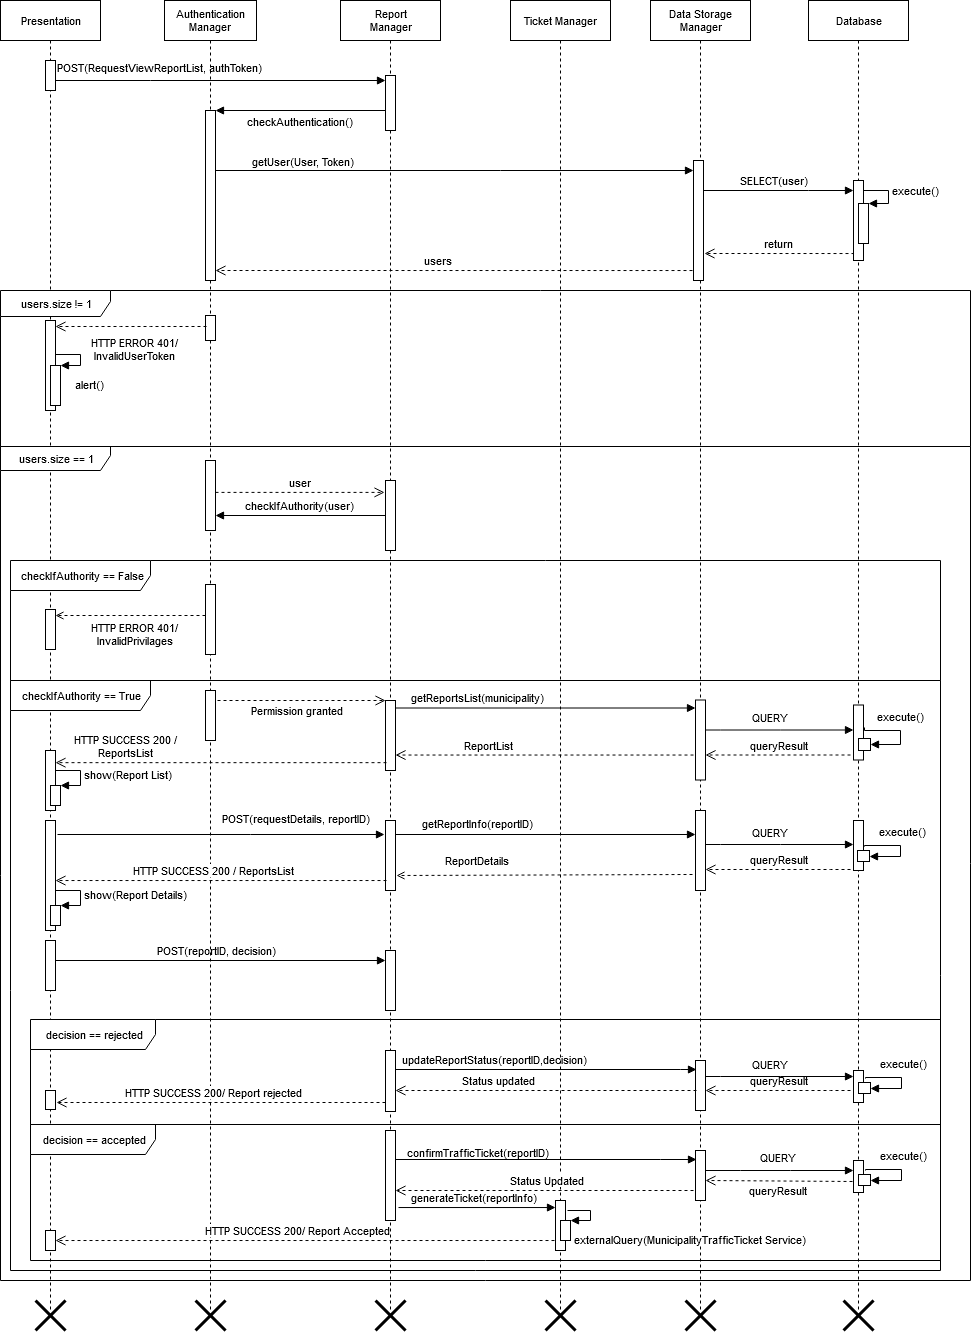
\includegraphics[scale=0.4]{Images/seq_gen_multa_def_ultimo2.png}
        \caption{Creation of a Traffic Ticket Runtime View}
\end{figure}

\subsubsection{Get Suggestions Runtime View}
In this sequence diagram is shown the Runtime when an Authority want to see new suggestions.\\
As usual the first step is the verification of the authentication and of the necessary privileges. After that, the Suggestions Manager cross the data of the reports done on Safestreets with the Municipality data, so it needs to view the Report List and to invoke the Municipality System API. After the cross operation has been performed, it obtains one o more new suggestions that will be stored in the Database and then returned to the Application Client to be shown to the Authority.
\begin{figure}[H]
          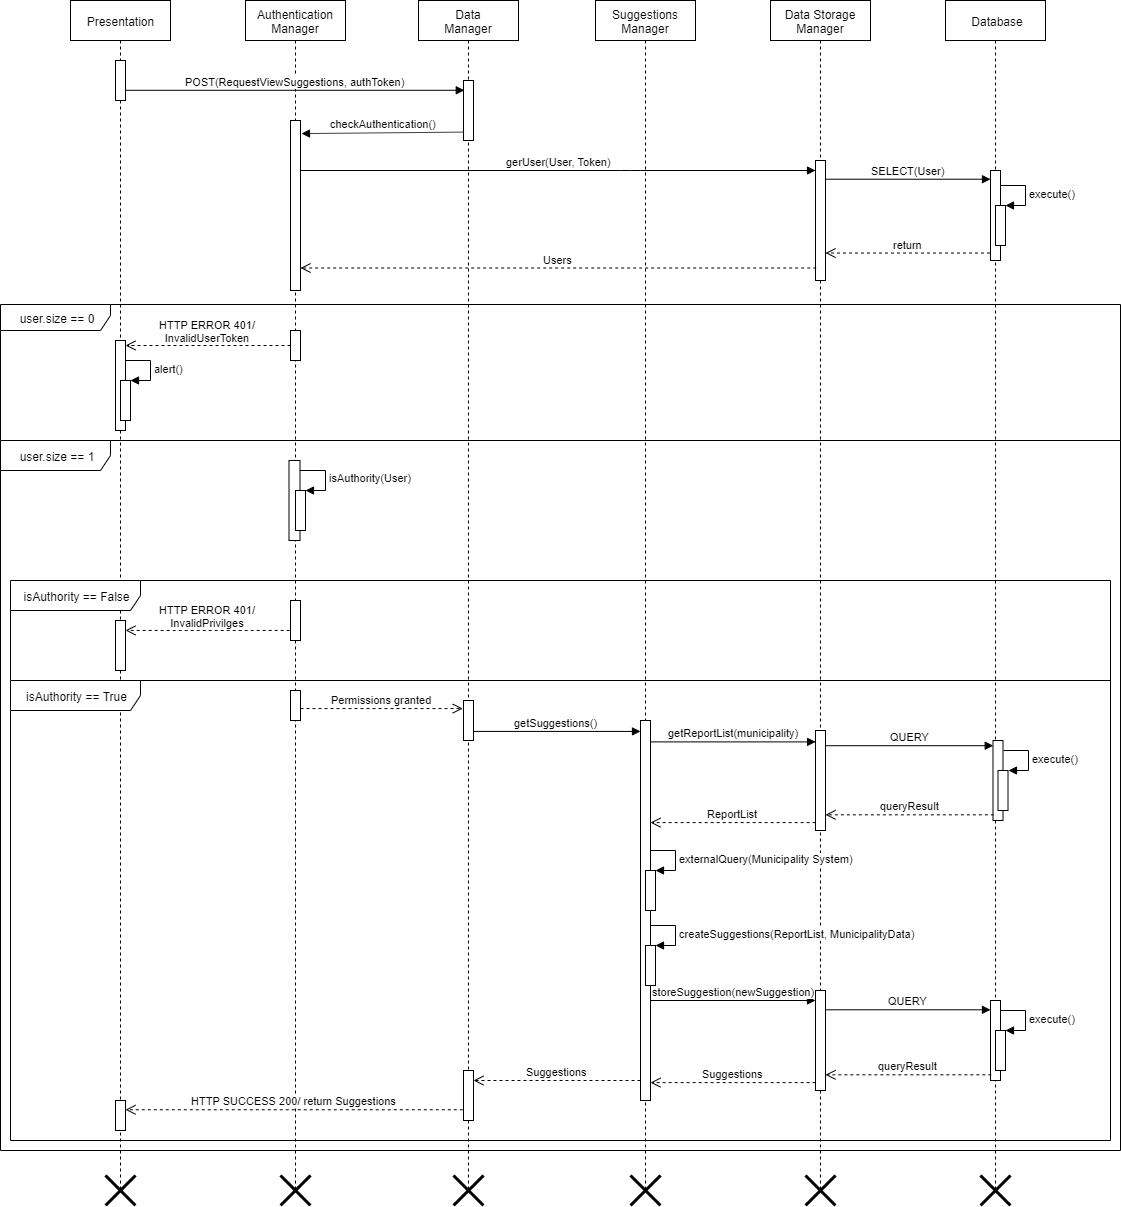
\includegraphics[scale=0.35]{Images/Seq_viewSuggestions.png}
        \caption{Request of Suggestions Runtime View}
\end{figure}

\subsubsection{Get Statistics Runtime View}
In this last sequence diagram is shown the Runtime behaviour of the Application when an Authority or a User want to see SafeStreets Statistics.\\
After the check of authentication (both User and Authority can see Statistics, but they must be logged in) the Data Manager sends the request to the Statitics Manager which take from the Database all the Reports and then extract information from them in order to generate statistics.\\
The final step is to send the generated statistics to the Application Client.
\begin{figure}[H]
          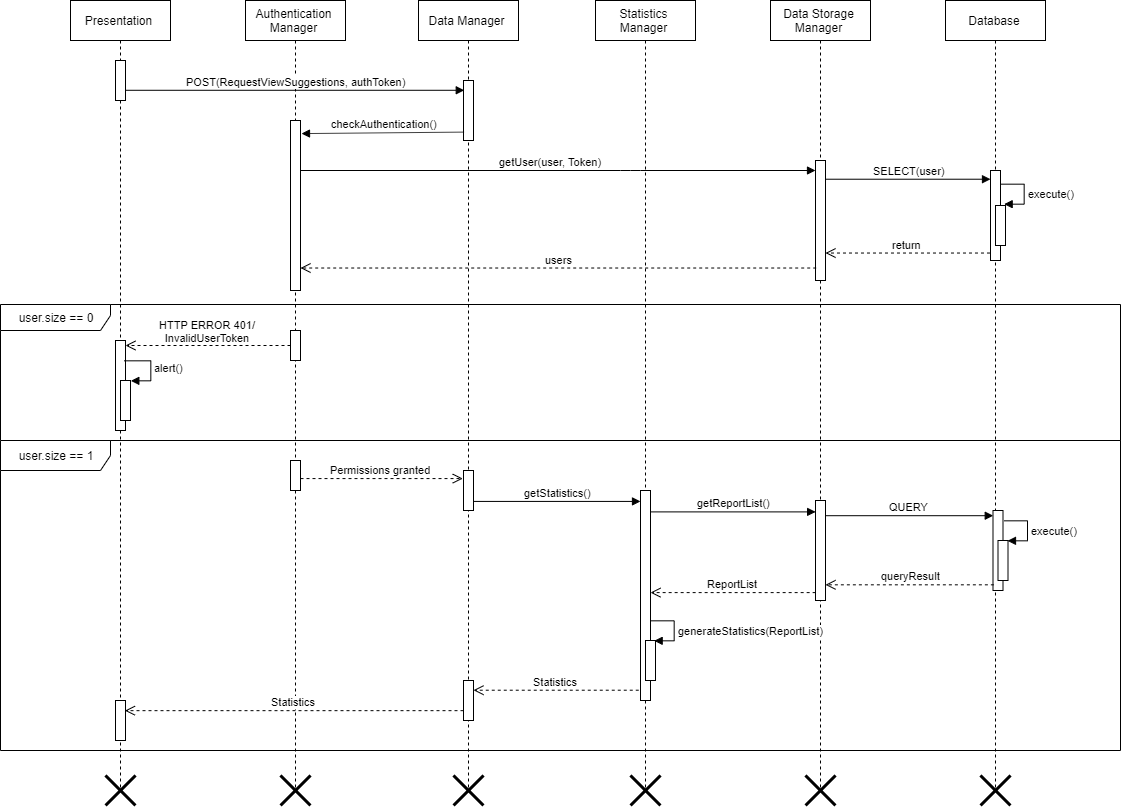
\includegraphics[scale=0.35]{Images/Seq_viewStatistics.png}
        \caption{Request of Statistics Runtime View}
\end{figure}
\newpage
\subsection{Component interfaces}
\textbf{Interface Diagram} 

\begin{figure}[H]
\centering
\advance\leftskip-6cm
          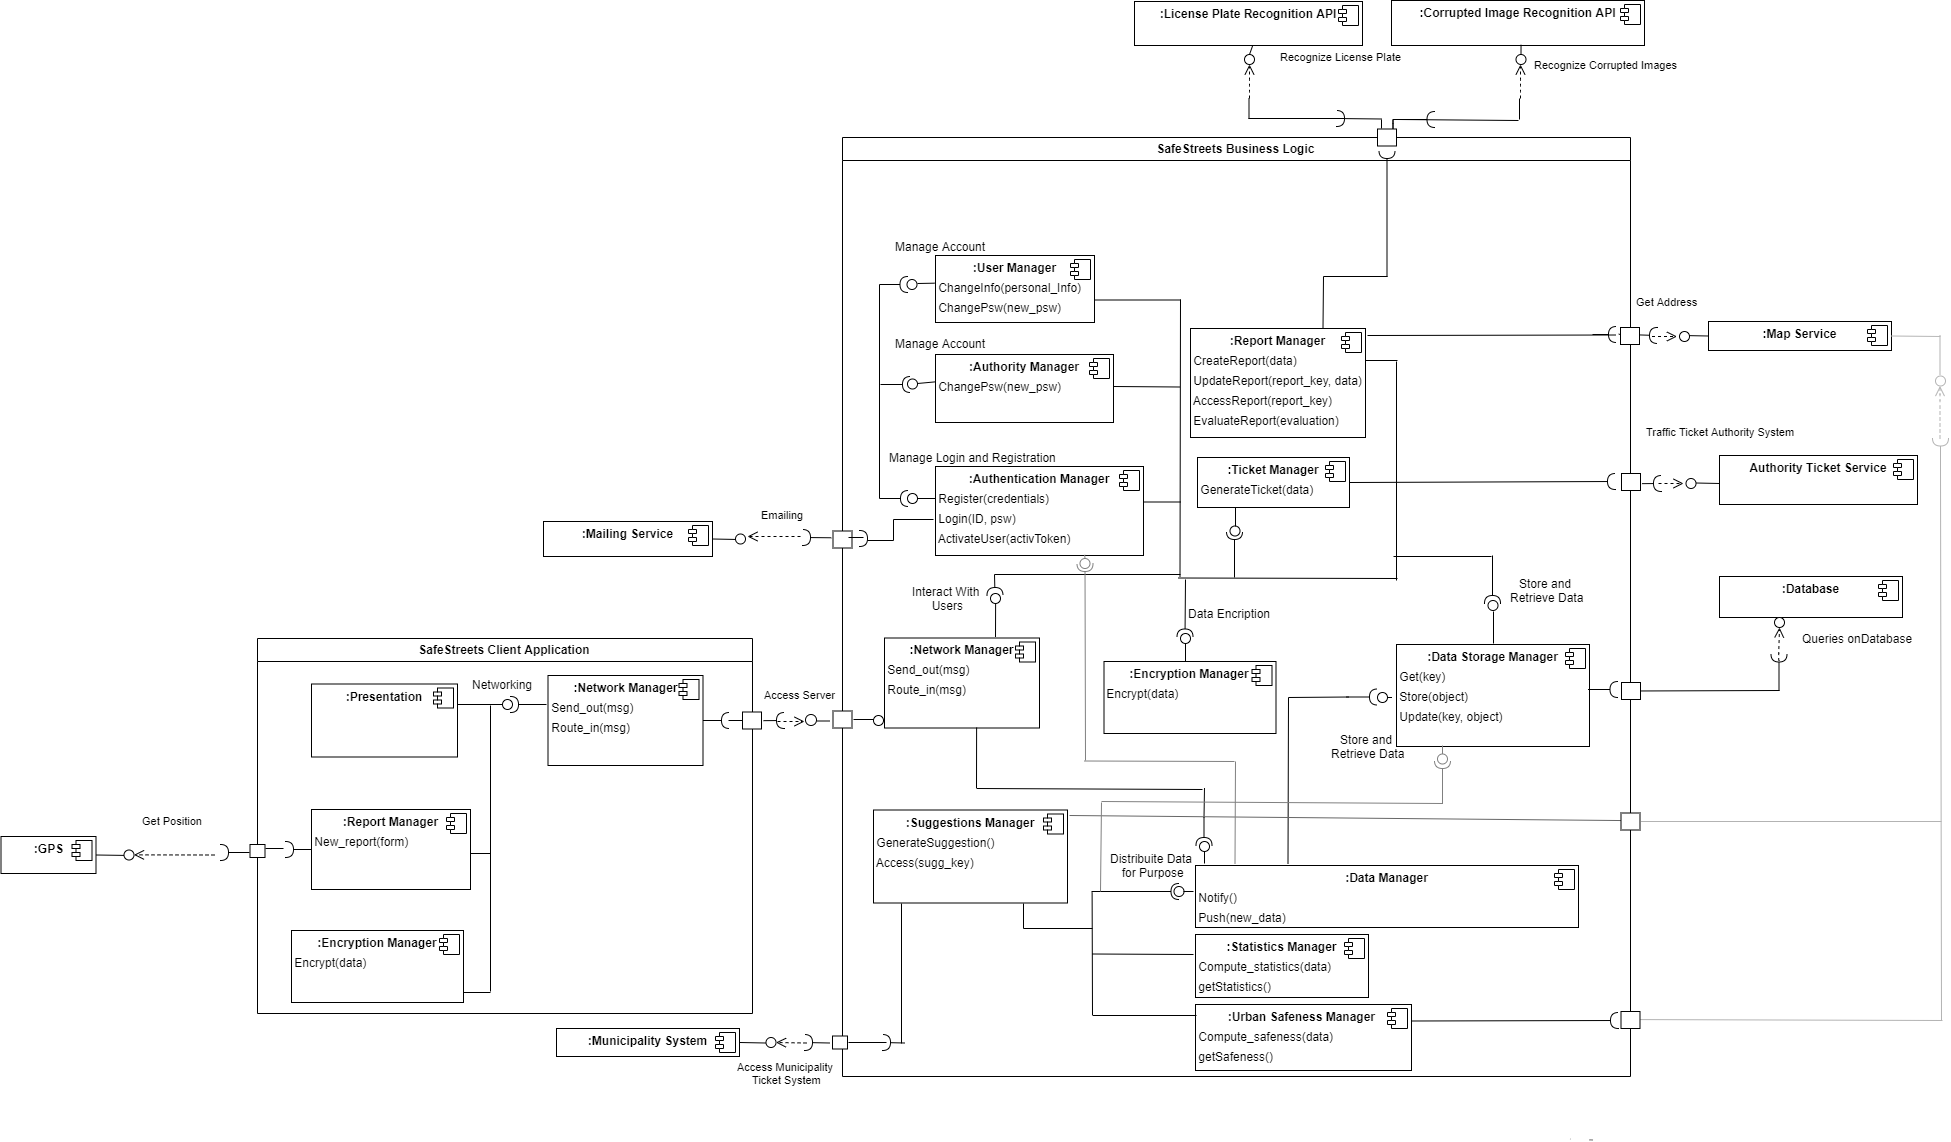
\includegraphics[width=1.5\textwidth,left]{Images/Component_interface.png}
        \caption{Component Interface diagram}
\end{figure}
\newpage
\textbf{REST API}
\begin{table}[H]
\begin{tabular}{|l|p{0.9\textwidth}|}
\hline
\textbf{Info}             & User register to the service                                                                           \\ \hline
\textbf{Endpoint}    &  /*auth/reg/User\\ \hline
\textbf{Method}         &   \textbf{POST}                                                                            \\ \hline

\textbf{Body}  &   email:[string] \newline
                   username:[string] \newline
                   password:[string] \newline 
                   full\_name:[string]
                    \\ \hline
                    
\textbf{Success} &  Code: 200 OK \newline
                    Content:\{\newline 
                    message: "successfully registered"\newline 
                    \}\\ \hline
\textbf{Error} &  Code: 400 \newline
                  Content:\{\newline
                  error:"data are not valid"\newline\}\newline
                  
                  Code: 422 \newline
                  Content:\{\newline
                  error:"this user is already registered"\newline\}\\\hline

\end{tabular}
\end{table}



%TABLE 2


\begin{table}[H]
\begin{tabular}{|l|p{0.9\textwidth}|}
\hline
\textbf{Info}             & User activates his/her account                                                                         \\ \hline
\textbf{Endpoint}    & /*auth/actv?activToken=[string] \\ \hline
\textbf{Method}         &   \textbf{GET}                                                                            \\ \hline

\textbf{Body}  &   \\ \hline
                    
\textbf{Success} &  Code: 200 OK \newline
                    Content:\{\newline 
                    message: "account successfully activated"\newline 
                    \}\\ \hline
\textbf{Error} &  Code: 401 \newline
                  Content:\{\newline
                  error:"account not authorized. Token not valid"\newline\}\newline
                  
                  Code: 422 \newline
                  Content:\{\newline
                  error:"this account is already activated"\newline\}\\\hline

\end{tabular}
\end{table}




%TABLE 3


\begin{table}[H]
\begin{tabular}{|l|p{0.9\textwidth}|}
\hline
\textbf{Info}             & User and Authority log in                                                                       \\ \hline
\textbf{Endpoint}    &  /*auth/login\\ \hline
\textbf{Method}         &   \textbf{POST}                                                                            \\ \hline

\textbf{Body}  &     username:[string] \newline
                   password:[string] 
              
                    \\ \hline
                    
\textbf{Success} &  Code: 200 OK \newline
                    Content:\{\newline 
                    message: "successfully logged in"\newline 
                    \}\\ \hline
\textbf{Error} &   Code: 400 \newline
                  Content:\{\newline
                  error:"data are not valid"\newline\}\newline
                  
                  Code: 401 \newline
                  Content:\{\newline
                  error:"account not activated"\newline\}\newline
                  
                  Code: 401 \newline
                  Content:\{\newline
                  error:"incorrect username or password "\newline\}\\\hline

\end{tabular}
\end{table}




%TABLE 4


\begin{table}[H]
\begin{tabular}{|l|p{0.9\textwidth}|}
\hline
\textbf{Info}             & User modify his/her account info                                                                      \\ \hline
\textbf{Endpoint}    &  /*User/Settings/info\\ \hline
\textbf{Method}         &   \textbf{POST}                                                                            \\ \hline

\textbf{Body}  &     activToken:[string] \newline
                   name:[string]\newline
                   surname:[string]\newline
              
                    \\ \hline
                    
\textbf{Success} &  Code: 200 OK \newline
                    Content:\{\newline 
                    message: "changes applied"\newline 
                    \}\\ \hline
\textbf{Error} &  Code: 400 \newline
                  Content:\{\newline
                  error:"data are not valid"\newline\}\newline
                  
                  Code: 403 \newline
                  Content:\{\newline
                  error:"User username and token don't match"\newline\}\newline
                  
                  Code: 404 \newline
                  Content:\{\newline
                  error:"User not found "\newline\}\\\hline

\end{tabular}
\end{table}




%TABLE 5



\begin{table}[H]
\begin{tabular}{|l|p{0.9\textwidth}|}
\hline
\textbf{Info}             & User accesses his/her account info                                                                      \\ \hline
\textbf{Endpoint}    &  /*User/Settings/info\\ \hline
\textbf{Method}         &   \textbf{GET}                                                                            \\ \hline

\textbf{Body}  &
                    \\ \hline
                    
\textbf{Success} &  Code: 200 OK \newline
                    Content:\{\newline 
                    name:[string]\newline
                 surname:[string]\newline
                 username:[string]\newline
                    \}\\ \hline
\textbf{Error} &  
                  Code: 403 \newline
                  Content:\{\newline
                  error:"User username and token don't match\newline\}\newline
                  
                  Code: 404 \newline
                  Content:\{\newline
                  error:"User not found "\newline\}\\\hline

\end{tabular}
\end{table}




%TABLE 6



\begin{table}[H]
\begin{tabular}{|l|p{0.9\textwidth}|}
\hline
\textbf{Info}             & Authority accesses his/her account info                                                                      \\ \hline
\textbf{Endpoint}    &  /*Autho/Settings/info\\ \hline
\textbf{Method}         &   \textbf{GET}                                                                            \\ \hline

\textbf{Body}  &
                    \\ \hline
                    
\textbf{Success} &  Code: 200 OK \newline
                    Content:\{\newline 
                    name:[string]\newline
                 surname:[string]\newline
                 username:[string]\newline
                 municipality:[string]\newline
                    \}\\ \hline
\textbf{Error} &  
                  Code: 403 \newline
                  Content:\{\newline
                  error:"Authority username and token don't match\newline\}\newline
                  
                  Code: 404 \newline
                  Content:\{\newline
                  error:"User not found "\newline\}\\\hline

\end{tabular}
\end{table}



%TABLE 7



\begin{table}[H]
\begin{tabular}{|l|p{0.9\textwidth}|}
\hline
\textbf{Info}             & User or Authority changes password                                                                    \\ \hline
\textbf{Endpoint}    &  /*User/Settings/credentials or /*Autho/Settings/credentials\\ \hline
\textbf{Method}         &   \textbf{POST}                                                                            \\ \hline

\textbf{Body}  & activToken:[string]\newline
oldPassword:[string]\newline
newPassword:[string]\newline
                    \\ \hline
                    
\textbf{Success} &  Code: 200 OK \newline
                    Content:\{\newline 
                    message:"password changed successfully"\newline
                    \}\\ \hline
\textbf{Error} &  Code: 400 \newline
                  Content:\{\newline
                  error:"new password not valid"\newline\}\newline
                  
                  Code: 400 \newline
                  Content:\{\newline
                  error:"old password not correct"\newline\}\newline
                  
                  Code: 403 \newline
                  Content:\{\newline
                  error:"username and token don't match"\newline\}\newline
                  
                  Code: 404 \newline
                  Content:\{\newline
                  error:"User not found "\newline\}\\\hline

\end{tabular}
\end{table}



%TABLE 8



\begin{table}[H]
\begin{tabular}{|l|p{0.9\textwidth}|}
\hline
\textbf{Info}             & A User sends a report                                                                   \\ \hline
\textbf{Endpoint}    &  /*report/create \\ \hline
\textbf{Method}         &   \textbf{POST}                                                                            \\ \hline

\textbf{Body}  & picture:[object]\newline
kindOfviolation:[int]\newline
GPS:[string]\newline
dateTime:[date]\newline
(optional) plate:[string]\newline
(optional) model:[string]\newline
(optional) brand:[string]\newline
(optional) color:[string]\newline
                    \\ \hline
                    
\textbf{Success} &  Code: 200 OK \newline
                    Content:\{\newline 
                    message:report created successfully"\newline
                    \}\\ \hline
\textbf{Error} &  Code: 400 \newline
                  Content:\{\newline
                  error:"inserted data not valid"\newline\}\newline
                  
                  Code: 400 \newline
                  Content:\{\newline
                  error:"missing some data"\newline\}\newline
                  
                  Code: 401 \newline
                  Content:\{\newline
                  error:"Not authorized." \newline\}
                  
                \\\hline

\end{tabular}
\end{table}



%TABLE 9



\begin{table}[H]
\begin{tabular}{|l|p{0.9\textwidth}|}
\hline
\textbf{Info}             & User views a list of his/her reports                                                              \\ \hline
\textbf{Endpoint}    &  /*report/access?authToken=[string] \\ \hline
\textbf{Method}         &   \textbf{GET}                                                                            \\ \hline

\textbf{Body}  & 
                    \\ \hline
                    
\textbf{Success} &  Code: 200 OK \newline
                    Content:\{\newline 
                    listOf:\{\newline
                    reportPreview:[object]\newline \}\newline
                    \}\\ \hline
\textbf{Error} &  
                \\\hline

\end{tabular}
\end{table}


    %TABLE 10


\begin{table}[H]
\begin{tabular}{|l|p{0.9\textwidth}|}
\hline
\textbf{Info}             & A User views one of his/her reports                                                              \\ \hline
\textbf{Endpoint}    &  /*report/access?reportKey[string]\&authToken=[string] \\ \hline
\textbf{Method}         &   \textbf{GET}                                                                            \\ \hline

\textbf{Body}  & 
                    \\ \hline
                    
\textbf{Success} &  Code: 200 OK \newline
                    Content:\{\newline 
                   picture:[file]\newline
         typeOfViolation:[string]\newline
                   GPS:[string]\newline
                   dateTime:[date]\newline
                   address:[string]\newline
                   plate:[string]\newline
                   (optional) model:[string]\newline
                   (optional) brand:[string]\newline
                   (optional) color:[string]\newline
                    \}\\ \hline
\textbf{Error} &  Code: 400 \newline
                  Content:\{\newline
                  error:"reportKey not valid"\newline\}\newline
                  
                  
                  Code: 401 \newline
                  Content:\{\newline
                  error:"Not authorized. Report owner doesn't correspond to token." \newline\}
                 
                  
                \\\hline

\end{tabular}
\end{table}



%TABLE 11



\begin{table}[H]
\begin{tabular}{|l|p{0.9\textwidth}|}
\hline
\textbf{Info}             & Authority views a list of reports of his/her municipality                                                              \\ \hline
\textbf{Endpoint}    &  /*report?authToken=[string] \\ \hline
\textbf{Method}         &   \textbf{GET}                                                                            \\ \hline

\textbf{Body}  & 
                    \\ \hline
                    
\textbf{Success} &  Code: 200 OK \newline
                    Content:\{\newline 
                    listOf:\{\newline
                    reportPreview:[object]\newline\}\newline
                    \}\\ \hline
\textbf{Error} &  
                \\\hline

\end{tabular}
\end{table}




%TABLE 12



\begin{table}[H]
\begin{tabular}{|l|p{0.9\textwidth}|}
\hline
\textbf{Info}             & An Authority evaluates a report                                                           \\ \hline
\textbf{Endpoint}    &  /*report/evaluate \\ \hline
\textbf{Method}         &   \textbf{POST}                                                                            \\ \hline

\textbf{Body}  &    reportKey:[string]\newline
                    authToken:[string]\newline
                    evaluation:[boolean]
                    \\ \hline
                    
\textbf{Success} &  Code: 200 OK \newline
                    Content:\{\newline 
                  message:"report evaluated."\newline
                    \}\\ \hline
\textbf{Error} &  Code: 400 \newline
                  Content:\{\newline
                  error:"reportKey not valid"\newline\}\newline
                  
                  Code: 401 \newline
                  Content:\{\newline
                  error:"Not authorized." \newline\}\newline
                  
                   Code: 422 \newline
                  Content:\{\newline
                  error:"report already evaluated." \newline
                  \}\newline
                  
                \\\hline

\end{tabular}
\end{table}




%TABLE 13



\begin{table}[H]
\begin{tabular}{|l|p{0.9\textwidth}|}
\hline
\textbf{Info}             & Authority views a list of suggestions for his/her municipality                                                               \\ \hline
\textbf{Endpoint}    &  /*suggestions?authToken=[string] \\ \hline
\textbf{Method}         &   \textbf{GET}                                                                            \\ \hline

\textbf{Body}  & 
                    \\ \hline
                    
\textbf{Success} &  Code: 200 OK \newline
                    Content:\{\newline 
                    listOf:\{\newline
                    suggestionPreview:[object]\newline
                    \}\newline
                    \}\\ \hline
                    
\textbf{Error} &  Code: 401 \newline
                  Content:\{\newline
                  error:"Not authorized." \newline\}\newline
                \\\hline

\end{tabular}
\end{table}




%TABLE 14



\begin{table}[H]
\begin{tabular}{|l|p{0.9\textwidth}|}
\hline
\textbf{Info}             & An Authority asks for a new suggestion                                                        \\ \hline
\textbf{Endpoint}    &  /*suggestion/create?authToken=[string] \\ \hline
\textbf{Method}         &   \textbf{GET}                                                                            \\ \hline

\textbf{Body}  & 
                    \\ \hline
                    
\textbf{Success} &  Code: 200 OK \newline
                    Content:\{\newline 
            suggestion:[string]\newline
            (optional) GPS:[string]\newline
        (optional) picture:[file]\newline
                    \}\\ \hline
\textbf{Error} &  
                 
                  Code: 401 \newline
                  Content:\{\newline
                  error:"Not authorized." \newline\}\newline
                 
                \\\hline

\end{tabular}
\end{table}




%TABLE 15



\begin{table}[H]
\begin{tabular}{|l|p{0.9\textwidth}|}
\hline
\textbf{Info}             & User or Authority asks for statistics                                                        \\ \hline
\textbf{Endpoint}    &  /*statistics/showStatistics?type=[int]\&startDate=[date] \newline \&endDate=[date]\&municipality=[string] \\ \hline
\textbf{Method}         &   \textbf{GET}                                                                            \\ \hline

\textbf{Body}  & 
                    \\ \hline
                    
\textbf{Success} &  Code: 200 OK \newline
                    Content:\{\newline 
            x:[setOfInt]\newline
            y:[setOfInt]\newline
                    \}\\ \hline
\textbf{Error} &  
                 
                  Code: 400 \newline
                  Content:\{\newline
                  error:"date is not valid" \newline\}\newline
                  
                   Code: 400 \newline
                  Content:\{\newline
                  error:"municipalitiy is not valid" \newline\}
                  
                \\\hline

\end{tabular}
\end{table}




%TABLE 16



\begin{table}[H]
\begin{tabular}{|l|p{0.9\textwidth}|}
\hline
\textbf{Info}             & User or Authority asks for safe/unsafe areas.                                                        \\ \hline
\textbf{Endpoint}    &  /*Safenessmanager/showSafeness?municipality=[string] \\ \hline
\textbf{Method}         &   \textbf{GET}                                                                            \\ \hline

\textbf{Body}  & 
                    \\ \hline
                    
\textbf{Success} &  Code: 200 OK \newline
                    Content:\{\newline 
            requestedAreaMap:[object]\newline
                    \}\\ \hline
\textbf{Error} &
                   Code: 400 \newline
                  Content:\{\newline
                  error:"municipality is not valid" \newline\}
                  
                \\\hline

\end{tabular}
\end{table}



\subsection{Selected architectural styles and patterns}
In this section are shown the most relevant architectural design choices, with also the explanation of their role and their advantages.\\

\noindent \textbf{Multi-tier Architecture}\\
The architecture chosen for the System is a \textit{multi-tier architecture}, composed by three tiers: \textit{Presentation tier}, \textit{Application tier} and \textit{Data Storage tier}.\\
These division guarantees that each tier only deals with a specific task, creating a flexible and reusable application. Furthermore this very slight dependence allows modification to a single layer without affect the others, so the overall maintenance of the System is much easier.\\
Going more in details, these are the functionalities of each single tier:

\begin{itemize}
    \item \textit{Presentation tier:} is the only tier directly accessible by the user and it display to him/her all the information received by the Application tier.
    It also allows the user to interact with the application by requiring the execution of specific actions.
    \item \textit{Application tier:} is the core of the application, because it controls the application functionalities.
    In our architecture it includes both the application servers and the reverse proxy, which is used to handle client requests and to balance the workload.
    \item \textit{Data Storage tier:} in this last tier is included the Database of the System, so it includes all the mechanism about data storage. Also this layer is the core of the System, not in terms of functionalities but in terms of importance, because it contains all the data of the application and so it's always invoked by the other tiers.\\
\end{itemize}

\noindent \textbf{REST}\\
The communication between the Client and the Application Server is done according to the REpresentational State Transfer (REST).\\
Data exchange is also made through the HTTP Protocol and using SSL to provide encryption of sensible data.\\
Using HTTP and complying with REST guidelines allows to provide clear and complete APIs to the Clients.\\\\

\noindent \textbf{Relational DBMS}\\
The Data Storage layer consists of a relational DBMS. The relational model is a widely used design and there are several valid options, both open source and not, for what concerns the choice of the Management System.

\begin{figure}[H]
          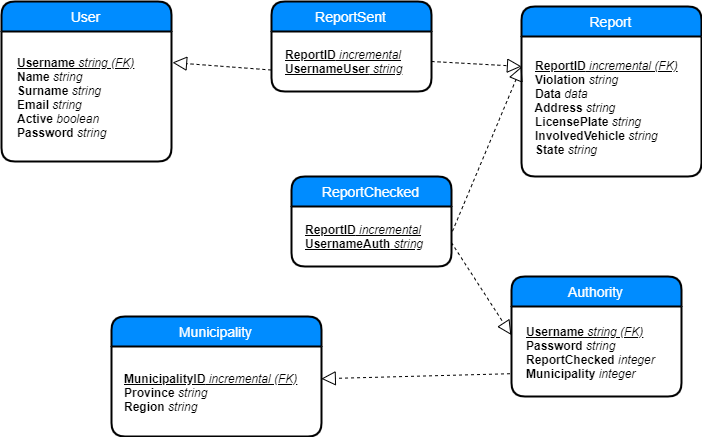
\includegraphics[scale=0.5]{Images/relationalDBMS.png}
        \caption{Database Schema Example}
\end{figure}

\subsection{Other design decisions}
\textbf{Firewall}\newline
Between the Reverse Proxy of the Application Server and the Internet, there is a Firewall with a default-deny policy, to apply a selective package filtering. There are a few kind of request that can be sent to the server, so it is an easy job to configure all the possible incoming requests in the default-deny Firewall, getting better results in term of security.\newline 

\noindent \textbf{Observer}\newline
An Observer Pattern has been implemented between the Data Manager and the Data Store Manager. Data Manager observes every new data that is added to the to Database. Then it notifies to Suggestion, Statistics and Urban Safeness Manager, depending on which of those is interested in the new data for their aims, pushing data to them.\\
This mechanism is used to make the Suggestions, Statistics and Urban Safeness Manager aware of each new data, so they can keep their information up to date.